% !TEX root = ../my_thesis.tex

\section{Ergebnisse}
 \label{sec:kapitel_4}

In dem vorliegenden Kapitel werden die Ergebnisse der durchgeführten Experimente präsentiert. Ein Evaluationsergebnis gibt in dieser Arbeit die Abweichung der Position in Metern und den Orientierungsfehler in Grad an. Ferner wird ein Evaluationsergebnis gegenüber Seinesgleichen anhand seines Positionsfehlers verglichen. Außerdem wird die Akkuratesse eines KNNs durch den Median aller Evaluationsergebnisse bestimmt. Im weiteren Verlauf dieses Kapitels werden zuerst die Reproduktionsergebnisse von \textit{BIM-PoseNet} \cite{acharyaBIMPoseNetIndoorCamera2019} angegeben und danach die Evaluationsergebnisse der trainierten Netzwerke dargestellt.

\subsection{Reproduktion der Ergebnisse von BIM-PoseNet}
Die Ergebnisse der Experimente von \citet{acharyaBIMPoseNetIndoorCamera2019} (\textit{BIM-PoseNet}), die das PoseNet Model mit den Gradientenbildern der karikaturistischen Daten (\textit{grad-cartoon}) sowie synthetischen Kantenbilder trainierten (\textit{grad-edge}) und anschließend mit den Gradientenbildern der realen Daten (\textit{grad-real}) evaluierten, konnten näherungsweise reproduziert werden (vgl. Tab. \ref{tab:reproduction}). Abweichend von \textit{BIM-PoseNet} wurden statt 1000 \textit{grad-real} Daten 600 \textit{grad-real} Daten evaluiert, weil zu derzeit 600 Evaluierungsbilder veröffentlicht waren. Der Trainingsprozess wurde pro Datensatztyp 5-mal wiederholt und die bessere Akkuratesse behalten. Eine exakte oder bessere Reproduktion der Ergebnisse ist durch Zufall bedingt und wurde in dieser Arbeit aus zeitlichen Gründen vernachlässigt. Tabelle \ref{tab:reproduction} präsentiert die Reproduktionergebnisse.


\begin{table}
	\centering
	\caption{Reproduktionsergebnisse. Abweichungen der Ergebnisse sind durch Zufall bedingt und können bei mehrfachem Wiederholen des Trainingsprozesses minimiert bzw. erhoben sowie verbessert werden. }
	\begin{tabularx}{1.0\textwidth}{X X X}
		\textbf{Netzwerk} \hspace{2cm} (Trainingsdatensatz) & \textbf{BIM-PoseNet} \hspace{2cm} (Position, Orientierung) & \textbf{Reproduktion} \hspace{2cm} (Position, Orientierung)\\
		\hline
	 \textit{grad-cartoon} & 2.63$m$, 6.99° & 2.57$m$, 10.52°\\
		\hline
		\textit{grad-edge} & 1.88$m$, 7.73° & 2.53$m$, 9.54°\\
	\end{tabularx}
	\label{tab:reproduction}
\end{table}





\subsection{Evaluation der trainierten KNNs}
Für alle synthetischen Datensätze einer Strecke wurde das Trainingsprozess 5-mal mit den korrespondierenden Gradientenbildern der Trainingsdaten separat wiederholt. Eine Evaluation folgte mit den Gradientenbildern der korrespondierenden synthetischen Evaluationsdaten (Evaluation 1). Eine weitere Evaluation der trainierten Netzwerke folgte mit den realen Evaluationsdaten der Strecke (Evaluation 2). Es wurden pro Strecke je Datensatztyp nur die beste Akkuratesse behalten. Tabellen \ref{tab:results_ic} bis \ref{tab:results_hs_stairs_down} geben die Akkuratesse der KNNs auf den jeweiligen Strecken an. 

Für ein besseres Verständnis der durch die Evaluierung mit den \textit{grad-real} Datensätzen resultierenden Akkuratesse wurden pro Strecke für die besten Netzwerke die bestimmten Positionen in der xy-Ebene dargestellt. Ebenso wurden pro Strecke die Positionsfehler in der xy-Ebene und die Orientierungsfehler auf der Gierachse der jeweiligen Evaluationsdaten dargestellt. Abbildungen \ref{fig:result_ic_loop} bis \ref{fig:result_hs_stairs_down} illustrieren die Evaluationsergebnisse. 
Ferner sollten die bei der Bestimmung des Hyperparameters $\beta$ ermittelten Akkuratessen als Referenzwerte für die Akkuratesse der jeweiligen Strecken dienen. Tabelle \ref{tab:results_traj_real} gibt die Referenzwerte und die durchschnittlichen Ergebnisse der Evaluationen pro Strecke an.

\subsubsection{IC-loop}
\label{subsubsec:ic_loop}

In diesem Experiment wurde der \textit{IC-loop} Datensatz verwendet. Die Evaluation bei einer durchschnittlichen Akkuratesse von 1.80$m$ in der Position und 8.05° in der Orientierung mit synthetischen Daten ergab mit den realen Daten eine durchschnittliche Akkuratesse von 24.38$m$, 61.24°. Eine Akkuratesse von 1.61$m$, 8.17° wurde mit synthetischen Daten beim Trainieren und Evaluieren durch den \textit{grad-cartoon} Datensatz erzielt. Bei der Evaluierung mit den Gradientenbildern der realen Evaluationsdaten wurde auf dem \textit{grad-photoreal} Netzwerk eine Akkuratesse von 16.68$m$, 73.25° erreicht (s. Tab. \ref{tab:results_ic}). 

Das \textit{grad-photoreal} Netzwerk bestimmte nur die Positionen aller \textit{grad-real} Evaluationsdaten auf einem ca. $30m \times 5m$ großen Teilbereich der unteren horizontalen Strecke (vgl. Abb. \ref{subfig:ic_fig2}). Daher wiesen Evaluationsdaten der kürzeren vertikalen sowie der obigen horizontalen Strecke die größten Positionsfehler auf (vgl. Abb. \ref{subfig:ic_fig4}). Ebenso bestimmte das Netzwerk größtenteils die Orientierung der Evaluationsdaten als die Aufnahmerichtung der unteren horizontalen Strecke (vgl. Abb. \ref{subfig:ic_fig6}).

\begin{table}
	\centering
	\caption{Evaluationsergebnisse von der \textit{IC-loop} Strecke. Die Akkuratesse der mit den jeweiligen Trainingsdaten trainierten Netzwerken werden angegeben. Diese Netzwerke wurden mit den korrespondierenden synthetischen Evaluationsdaten und jeweils mit den realen Evaluationsdaten evaluiert.}
		\begin{tabularx}{1.0\textwidth}{X >{\RaggedRight}X >{\RaggedRight}X}
		\textbf{Trainingsdatensatz} \hspace{2cm} (Gradientenbild) & \textbf{synthetische Daten} \hspace{2cm} (Position, Orientierung) & \textbf{reale Daten} \hspace{2cm} (Position, Orientierung)\\
		\hline
			\textit{grad-cartoon} & 1.61$m$, 8.17° & 23.56$m$, 51.30°\\
			\hline
			\textit{grad-edge} & 2.00$m$, 8.29° & 32.91$m$, 59.17°\\
			\hline
			\textit{grad-photoreal} & 1.80$m$, 7.70° & 16.68$m$, 73.25°\\
			\hhline{===}
			$\emptyset$ Durchschnitt & 1.80$m$, 8.05° & 24.38$m$, 61.24°\\
		\end{tabularx}
	\label{tab:results_ic}
\end{table}



\begin{figure}
	\setlength\extrarowheight{-15pt}
	\centering
	\begin{tabularx}{0.9\textwidth}{>{\centering\arraybackslash}p{0.05\textwidth} X}
		\subcaption{} \label{subfig:ic_fig2} & \imagetop{ 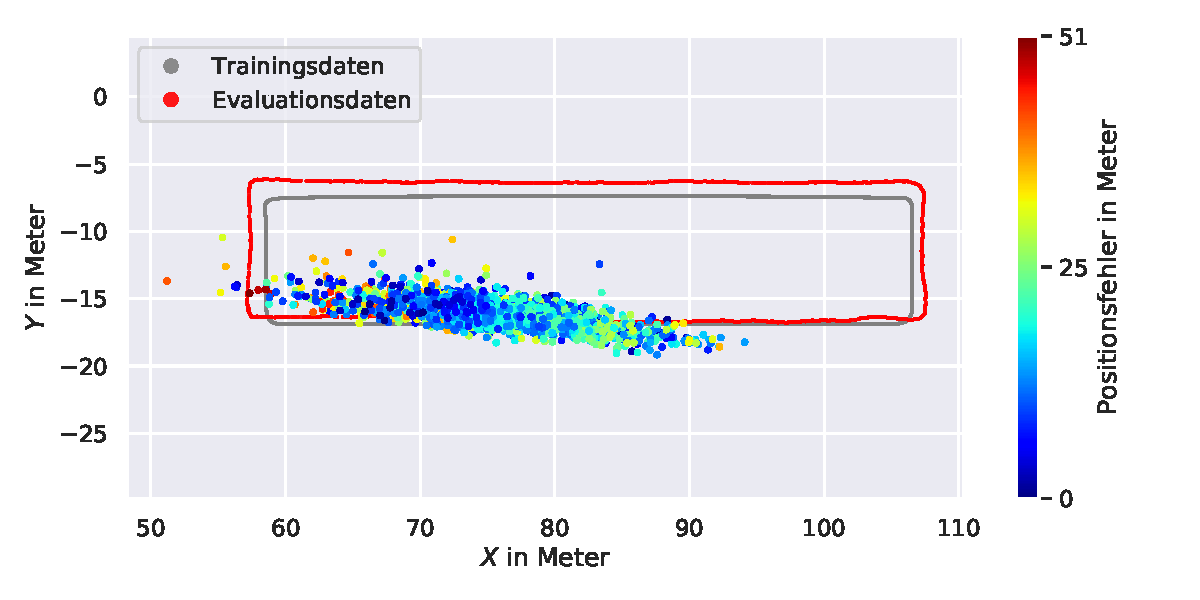
\includegraphics[width=1.0\linewidth]{images/results/ic_cycl/resultsfig_2.pdf} }\\
		\subcaption{} \label{subfig:ic_fig4} & \imagetop{ 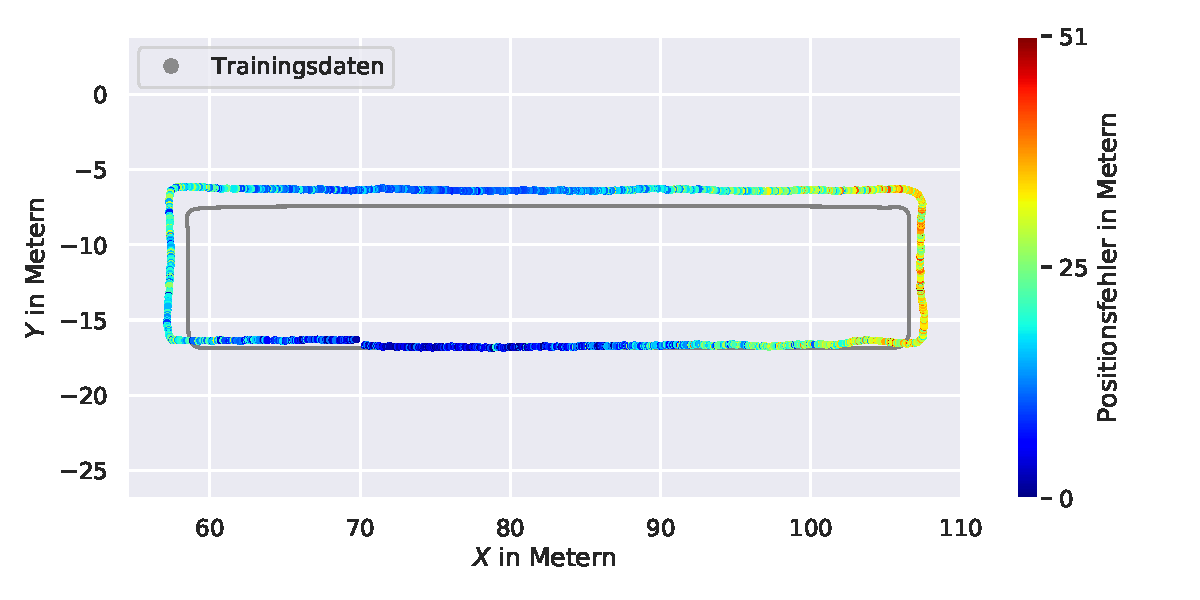
\includegraphics[width=1.0\linewidth]{images/results/ic_cycl/resultsfig_4.pdf} }\\
		\subcaption{} \label{subfig:ic_fig6} & \imagetop{ 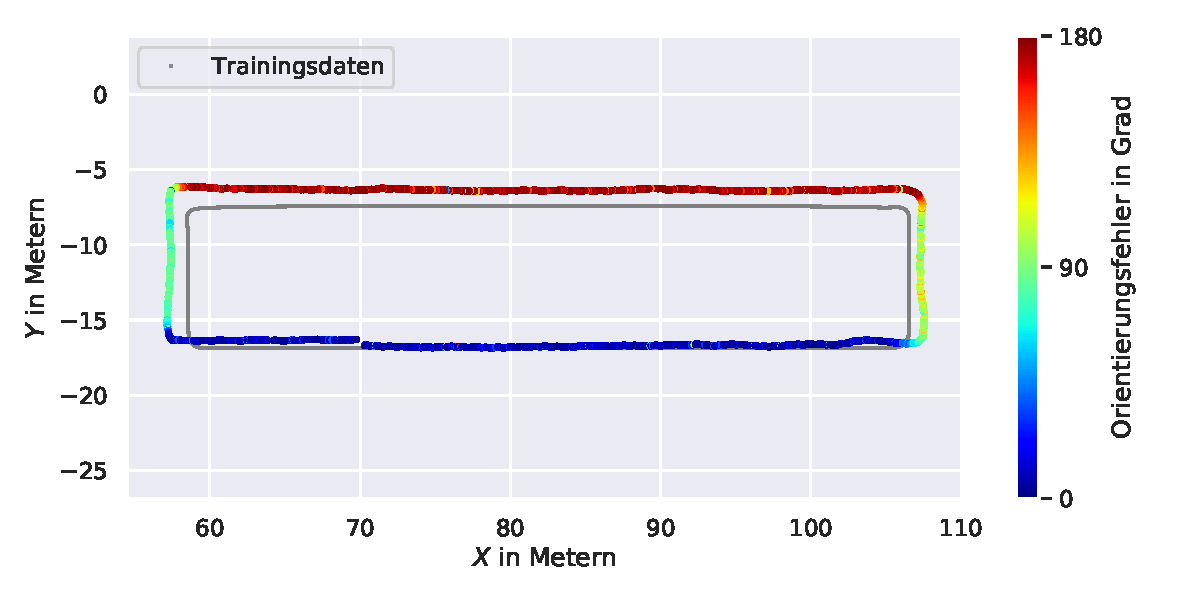
\includegraphics[width=1.0\linewidth]{images/results/ic_cycl/resultsfig_6.pdf} }\\
	\end{tabularx}
	\caption{Visualisierung der Evaluationsergebnisse der \textit{IC-loop} Strecke (s. Abb. \ref{subfig:traj_ic}). Die Evaluation folgte mit den Gradietenbildern der realen Daten auf dem mit \textit{grad-photoreal} trainierten Netzwerk. \subref{subfig:ic_fig2} illustriert die von dem KNN bestimmten Positionen auf der xy-Ebene. Der Positionsfehler in der xy-Ebene und der Orientierungsfehler auf der Gierachse der jeweiligen Evaluationsdaten werden in \subref{subfig:ic_fig4} und \subref{subfig:ic_fig6} dargestellt.}
	\label{fig:result_ic_loop}
\end{figure}


\subsubsection{HS-gamma}
\label{subsubsec:hs_gamma}
Ein weiteres Experiment folgte mit dem \textit{HS-gamma} Datensatz. Die Evaluation bei einer durchschnittlichen Akkuratesse von 1.17$m$, 9.26° mit synthetischen Daten ergab mit den realen Daten eine durchschnittliche Akkuratesse von 9.67$m$, 32.10°. Trainiert und evaluiert mit nur synthetischen Daten wurde durch dem \textit{grad-cartoon} Datensatz eine Akkuratesse von 1.00$m$, 9.92° erzielt. Die Evaluierung mit den \textit{grad-real} Evaluationsdaten auf dem \textit{grad-cartoon} Netzwerk führte zu einer Akkuratesse von 8.60$m$, 19.59° (s. Tab. \ref{tab:results_hs_gamma}). 


Das \textit{grad-cartoon} Netzwerk bestimmte überwiegend die Positionen aller \textit{grad-real} Evaluationsdaten auf der linken horizontalen Strecke auf einem ca. $20m \times 5m$ großen Teilbereich (vgl. Abb. \ref{subfig:hs_gamma_fig2}). Deshalb wiesen die Evaluationsdaten der linken horizontalen Strecke die geringsten Positionsfehler auf. Zudem zeigten die Evaluationsdaten des zum Ausgangspunkt optisch ähnlichen Flures die größten Positionsfehler auf (vgl. Abb. \ref{subfig:ic_fig4}). Ebenso bestimmte das oben erwähnte Netzwerk mehrheitlich die Orientierung der Evaluationsdaten als die Orientierung der dominierenden Aufnahmerichtung. Daher waren die größten Orientierungsfehler bei den Evaluationsdaten der Schlaufe sowie der vertikal verlaufenden Strecke aufzufinden (vgl. Abb. \ref{subfig:ic_fig4}). 


\begin{table}
	\centering
	\caption{Evaluationsergebnisse von der \textit{HS-gamma} Strecke. Die Akkuratesse der mit den jeweiligen Trainingsdaten trainierten Netzwerken wird angegeben. Diese Netzwerke wurde mit den korrespondierenden synthetischen Evaluationsdaten und jeweils mit den realen Evaluationsdaten evaluiert.}
	\begin{tabularx}{1.0\textwidth}{X >{\RaggedRight}X >{\RaggedRight}X}
		\textbf{Netzwerk} \hspace{2cm} (Trainingsdatensatz) & \textbf{synthetische Daten} \hspace{2cm} (Position, Orientierung) & \textbf{reale Daten} \hspace{2cm} (Position, Orientierung)\\
	\hline
		\textit{grad-cartoon} & 1.00$m$, 9.92° & 8.60$m$, 19.59°\\
		\hline
		\textit{grad-edge} & 1.07$m$, 8.69° & 10.15$m$, 35.11°\\
		\hline
		\textit{grad-photoreal} & 1.45$m$, 9.17° & 10.27$m$, 41.60°\\
		\hhline{===}
		$\emptyset$ Durchschnitt & 1.17$m$, 9.26° & 9.67$m$, 32.10°\\
	\end{tabularx}
	\label{tab:results_hs_gamma}
\end{table}

\begin{figure}
	\setlength\extrarowheight{-15pt}
	\centering
	\begin{tabularx}{0.9\textwidth}{>{\centering\arraybackslash}p{0.05\textwidth} X}
		\subcaption{} \label{subfig:hs_gamma_fig2} & \imagetop{ 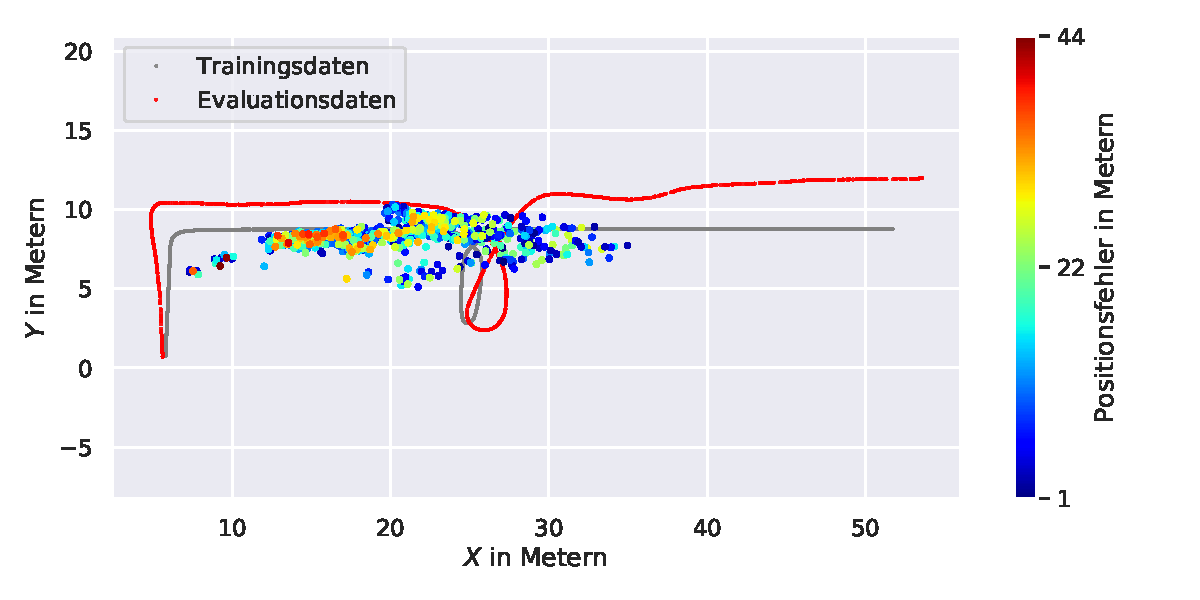
\includegraphics[width=1.0\linewidth]{images/results/hs_gamma/resultsfig_2.pdf} }\\
		\subcaption{} \label{subfig:hs_gamma_fig4} & \imagetop{ 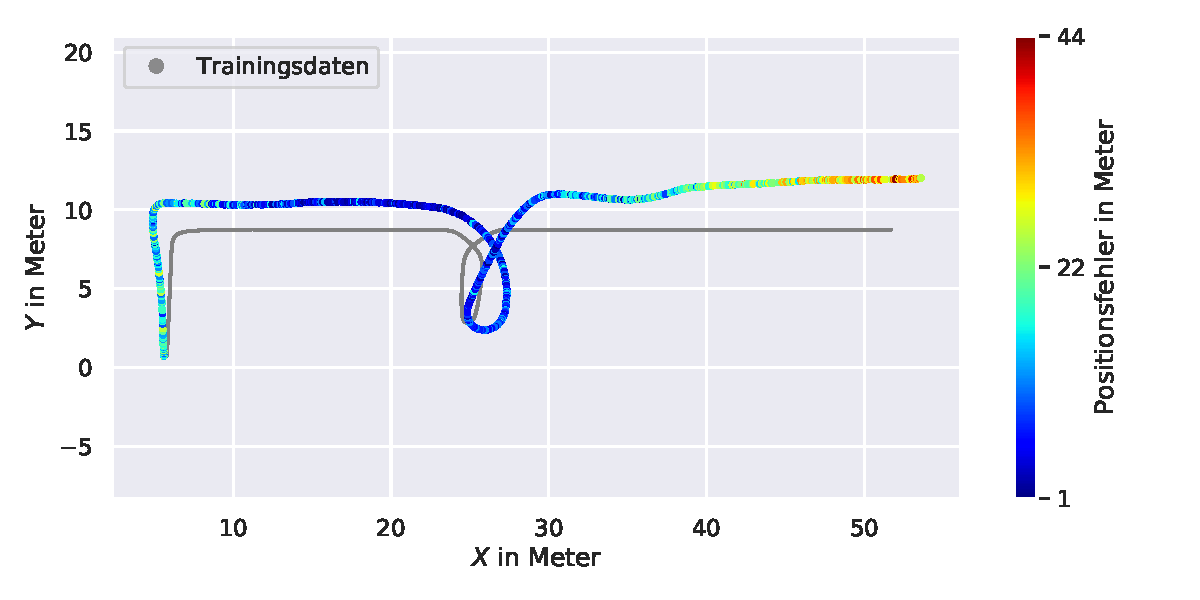
\includegraphics[width=1.0\linewidth]{images/results/hs_gamma/resultsfig_4.pdf} }\\
		\subcaption{} \label{subfig:hs_gamma_fig6} & \imagetop{ 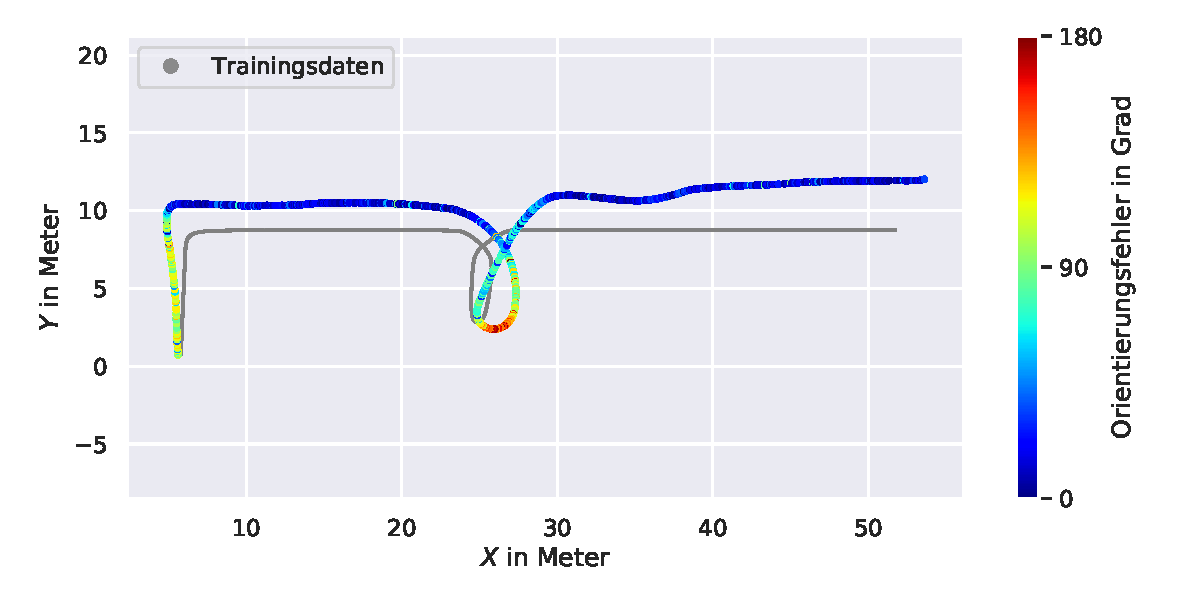
\includegraphics[width=1.0\linewidth]{images/results/hs_gamma/resultsfig_6.pdf} }\\
	\end{tabularx}
	\caption{Visualisierung der Evaluationsergebnisse der \textit{HS-gamma} Strecke (s. Abb. \ref{subfig:traj_hs_gamma}). Die Evaluation folgte mit den Gradietenbildern der realen Daten auf dem mit \textit{grad-cartoon} trainierten Netzwerk. \subref{subfig:hs_gamma_fig2} illustriert die von dem KNN bestimmten Positionen auf der xy-Ebene. Der Positionsfehler der xy-Ebene und der Orientierungsfehler auf der Gierachse der jeweiligen Evaluationsdaten werden in \subref{subfig:hs_gamma_fig4} und \subref{subfig:hs_gamma_fig6} dargestellt.}
	\label{fig:result_hs_gamma}
\end{figure}

\subsubsection{HS-stairs-up}
\label{subsubsec:hs_stairs_up}

Weiterhin wurde ein Experiment mit dem \textit{HS-stairs-up} Datensatz durchgeführt. Die Evaluation bei einer durchschnittlichen Akkuratesse von 0.85$m$, 8.07° mit synthetischen Daten ergab mit den realen Daten eine durchschnittliche Akkuratesse von 4.75$m$, 56.15°. Ausschließlich mit synthetischen Daten wurde eine Akkuratesse von 0.82$m$, 7.76° durch die \textit{grad-cartoon} Daten erzielt. Bei der Evaluierung mit den Gradientenbildern der realen Evaluationsdaten wurde eine Akkuratesse von 4.33$m$, 51.64° durch das \textit{grad-edge} Netzwerk erreicht (s. Tab. \ref{tab:results_hs_stairs_up}). 

Die vom \textit{grad-edge} Netzwerk bestimmten Positionen aller \textit{grad-real} Evaluationsdaten lagen mehrheitlich zwischen dem unteren und oberen Treppenlauf (vgl. Abb. \ref{subfig:hs_up_fig3}). Deshalb waren die größten Positionsfehler bei den Evaluationsdaten des Treppenabsatzes aufzufinden. Ebenso waren bei den Evaluationsdaten des unteren und oberen Treppenlaufes abwechselnd größere Positionsfehler zu erkennen. Hierbei wiesen die Evaluationsdaten des oberen Treppenlaufes häufiger einen größeren Positionsfehler auf als die des Unteren (vgl. Abb. \ref{subfig:hs_up_fig5}). Die Orientierung der Evaluationsdaten des oberen Treppenlaufes wurden überwiegend als die Orientierung der Evaluationsdaten des unteren Treppenlaufes bestimmt. Ebenso waren bei den Evaluationsdaten der Treppenläufe abwechselnd in der entgegengesetzten Orientierung Fehler zu erkennen (vgl. Abb. \ref{subfig:hs_up_fig7}).

\begin{table}
	\centering
	\caption{Evaluationsergebnisse von der Strecke \textit{HS-stairs-up} (s. Abb. \ref{subfig:traj_hs-up}). Die Akkuratesse der mit den jeweiligen Trainingsdaten trainierten Netzwerken werden angegeben. Diese Netzwerke wurden mit den korrespondierenden synthetischen Evaluationsdaten und jeweils mit den realen Evaluationsdaten evaluiert.}
	\begin{tabularx}{1.0\textwidth}{X >{\RaggedRight}X >{\RaggedRight}X}
		\textbf{Netzwerk} \hspace{2cm} (Trainingsdatensatz) & \textbf{synthetische Daten} \hspace{2cm} (Position, Orientierung) & \textbf{reale Daten} \hspace{2cm} (Position, Orientierung)\\
		\hline
		\textit{grad-cartoon} & 0.82$m$, 7.76° & 4.77$m$, 23.43°\\
		\hline
		\textit{grad-edge} & 0.82$m$, 8.48° & 4.33$m$, 51.64°\\
		\hline
		\textit{grad-photoreal} & 0.92$m$, 7.98° & 5.16$m$, 93.38°\\
		\hhline{===}
		$\emptyset$ Durchschnitt & 0.85$m$, 8.07° & 4.75$m$, 56.15°\\
	\end{tabularx}
	\label{tab:results_hs_stairs_up}
\end{table}


\begin{figure}
	\setlength\extrarowheight{-15pt}
	\centering
	\begin{tabularx}{0.9\textwidth}{>{\centering\arraybackslash}p{0.05\textwidth} X}
		\subcaption{} \label{subfig:hs_up_fig3} & \imagetop{ 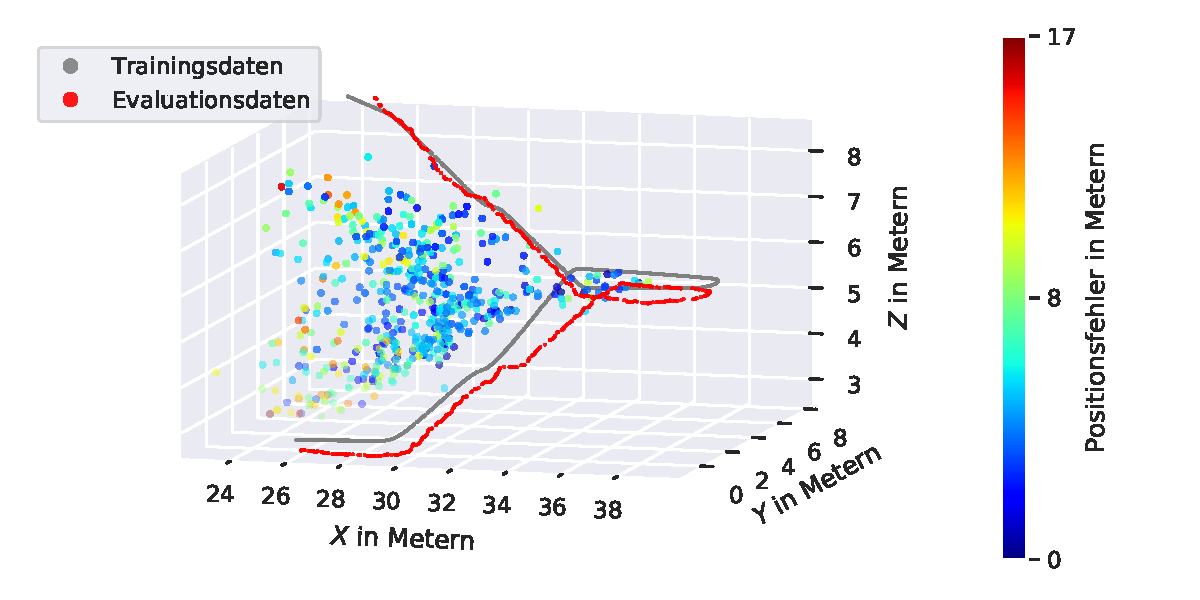
\includegraphics[width=1.0\linewidth]{images/results/hs_up/resultsfig_3.pdf} }\\
		\subcaption{} \label{subfig:hs_up_fig5} & \imagetop{ 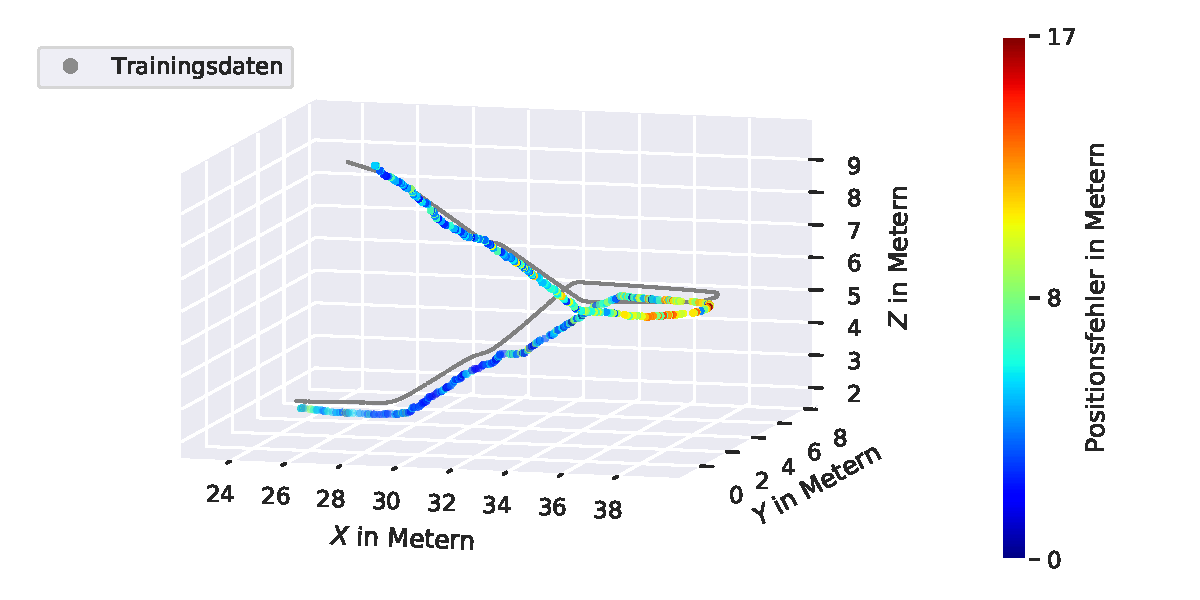
\includegraphics[width=1.0\linewidth]{images/results/hs_up/resultsfig_5.pdf} }\\
		\subcaption{} \label{subfig:hs_up_fig7} & \imagetop{ 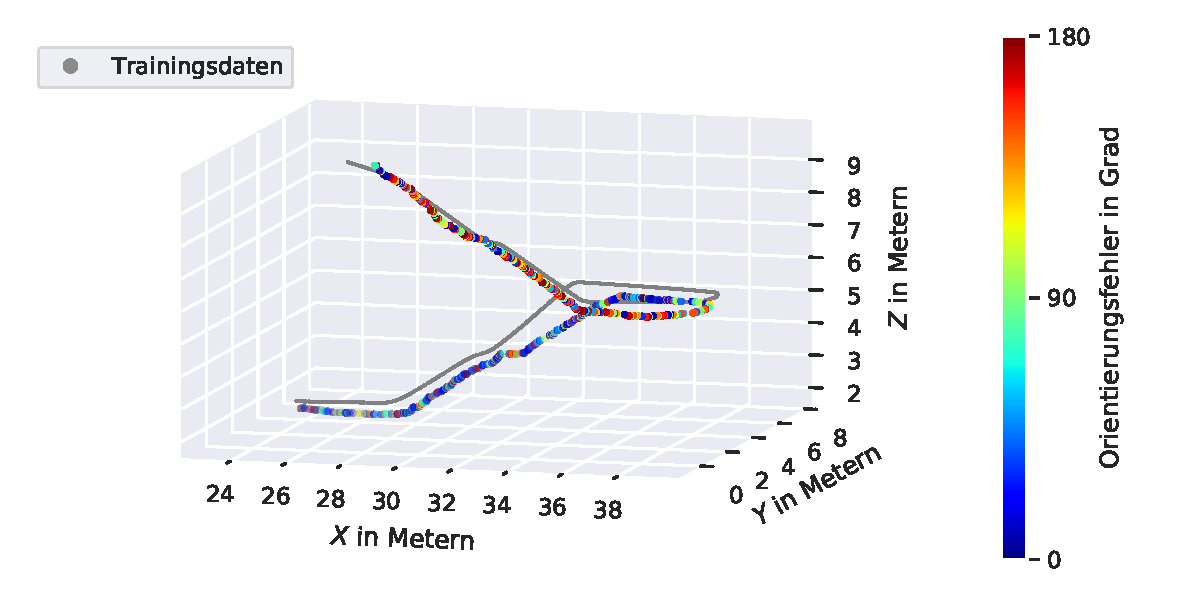
\includegraphics[width=1.0\linewidth]{images/results/hs_up/resultsfig_7.pdf} }\\
	\end{tabularx}
	\caption{Visualisierung der Evaluationsergebnisse der \textit{HS-stairs-up} Strecke. Die Evaluation folgte mit den Gradietenbildern der realen Daten auf dem mit \textit{grad-edge} trainierten Netzwerk. \subref{subfig:hs_up_fig3} illustriert die von dem KNN bestimmten Positionen auf der xy-Ebene. Der Positionsfehler in der xy-Ebene und der Orientierungsfehler auf der Gierachse der jeweiligen Evaluationsdaten werden in \subref{subfig:hs_up_fig5} und \subref{subfig:hs_up_fig7} dargestellt.} 
	\label{fig:result_hs_stairs_up}
\end{figure}


\subsubsection{HS-stairs-down}
\label{subsubsec:hs_stairs_down}



Zuletzt wurde ein Experiment mit dem \textit{HS-stairs-down} Datensatz durchgeführt. Die Evaluation bei einer durchschnittlichen Akkuratesse von 0.93$m$, 8.03° mit synthetischen Daten ergab mit den realen Daten eine durchschnittliche Akkuratesse von 5.01$m$, 49.29°. Nur mit synthetischen Daten beim Trainieren und Evaluieren wurde eine Akkuratesse von 0.85$m$, 7.50° durch die \textit{grad-edge} Daten erzielt. Die Evaluierung mit den \textit{grad-real} Evaluationsdaten auf dem mit \textit{grad-cartoon} trainierten Netzwerk führte zur einer Akkuratesse von 4.20$m$, 47.83° (s. Tab. \ref{tab:results_hs_stairs_down}). 

Das mit \textit{grad-cartoon} trainierte Netzwerk bestimmte die Positionen aller \textit{grad-real} Evaluationsdaten gleichermaßen wie im Unterabschnitt \ref{subsubsec:hs_stairs_up} zwischen dem unteren und oberen Treppenlauf (vgl. Abb. \ref{subfig:hs_down_fig3}). Deshalb waren hierbei genauso die größten Positionsfehler bei den Evaluationsdaten des Treppenabsatzes aufzufinden. Ebenso waren bei den Evaluationsdaten des unteren und oberen Treppenlaufes abwechselnd größere Positionsfehler zu erkennen. Diesmal wiesen die Evaluationsdaten des unteren Treppenlaufes häufiger einen größeren Positionsfehler auf (vgl. Abb. \ref{subfig:hs_down_fig5}). Im Vergleich zu \textit{HS-stairs-up} \ref{subsubsec:hs_stairs_up} ist in der Abbildung \ref{subfig:hs_down_fig7} entlang der Treppenläufe eine stärkere Abwechslung der Orientierungsfehler zu erkennen.

\begin{table}
	\centering
	\caption{Evaluationsergebnisse von der Strecke \textit{HS-stairs-down} (s. Abb. \ref{subfig:traj_hs-down}). Die Akkuratesse der mit den jeweiligen Trainingsdaten trainierten Netzwerken werden angegeben. Diese Netzwerke wurden mit den korrespondierenden synthetischen Evaluationsdaten und jeweils mit den realen Evaluationsdaten evaluiert.}
	\begin{tabularx}{1.0\textwidth}{X >{\RaggedRight}X >{\RaggedRight}X}
		\textbf{Netzwerk} \hspace{2cm} (Trainingsdatensatz) & \textbf{synthetische Daten} \hspace{2cm} (Position, Orientierung) & \textbf{reale Daten} \hspace{2cm} (Position, Orientierung)\\
		\hline
		\textit{grad-cartoon} & 0.91$m$, 8.01° & 4.20$m$, 47.83°\\
		\hline
		\textit{grad-edge} & 0.85$m$, 7.50° & 5.59$m$, 67.34°\\
		\hline
		\textit{grad-photoreal} & 1.02$m$, 8.57° & 5.25$m$, 32.70°\\
		\hhline{===}
		$\emptyset$ Durchschnitt & 0.93$m$, 8.03° & 5.01$m$, 49.29°\\
	\end{tabularx}
	\label{tab:results_hs_stairs_down}
\end{table}


\begin{figure}
	\setlength\extrarowheight{-15pt}
	\centering
	\begin{tabularx}{0.9\textwidth}{>{\centering\arraybackslash}p{0.05\textwidth} X}
		\subcaption{} \label{subfig:hs_down_fig3} & \imagetop{ 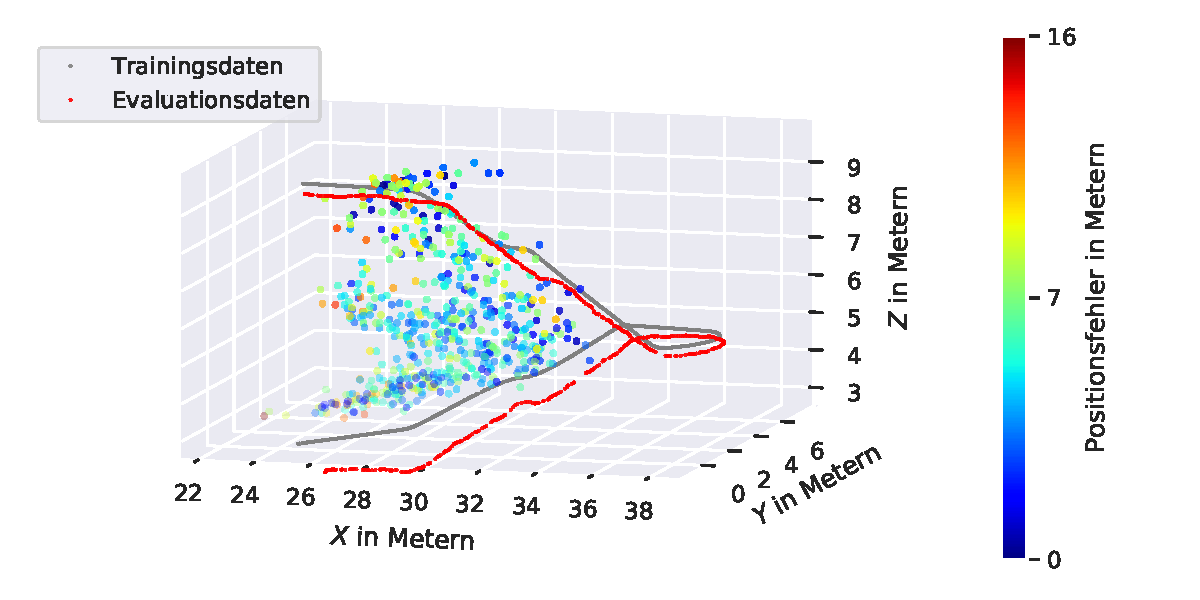
\includegraphics[width=1.0\linewidth]{images/results/hs_down/resultsfig_3.pdf} }\\
		\subcaption{} \label{subfig:hs_down_fig5} & \imagetop{ 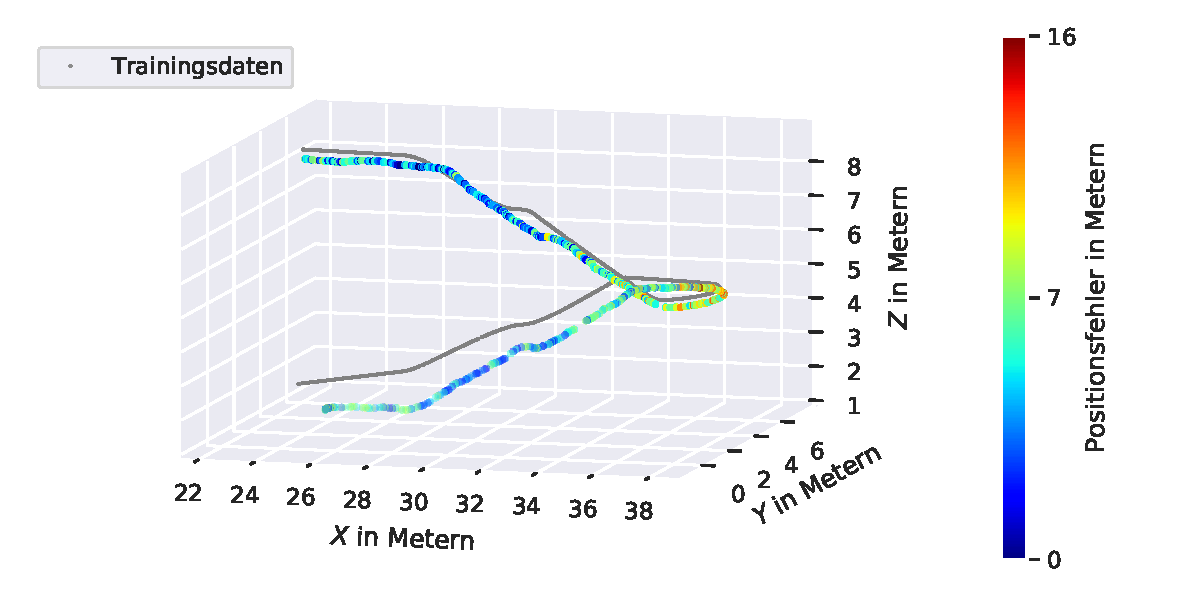
\includegraphics[width=1.0\linewidth]{images/results/hs_down/resultsfig_5.pdf} }\\
		\subcaption{} \label{subfig:hs_down_fig7} & \imagetop{ 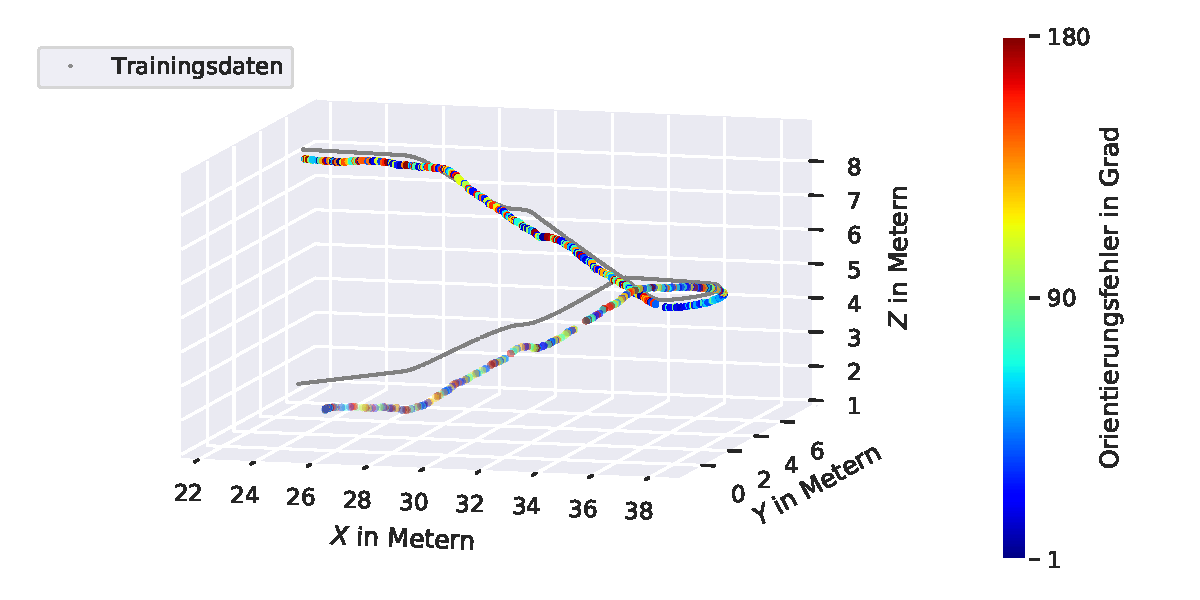
\includegraphics[width=1.0\linewidth]{images/results/hs_down/resultsfig_7.pdf} }\\
	\end{tabularx}
	\caption{Visualisierung der Evaluationsergebnisse der Strecke \textit{HS-stairs-down}. Die Evaluation folgte mit den Gradietenbildern der realen Daten auf dem mit \textit{grad-cartoon} trainierten Netzwerk. \subref{subfig:hs_down_fig3} illustriert die von dem KNN bestimmten Positionen auf der xy-Ebene. Der Positionsfehler in der xy-Ebene und der Orientierungsfehler auf der Gierachse der jeweiligen Evaluationsdaten werden in \subref{subfig:hs_down_fig5} und \subref{subfig:hs_down_fig7} dargestellt.}
	\label{fig:result_hs_stairs_down}
\end{figure}




\begin{table}
	\centering
	\caption{Zusammenfassung der Evaluationsergebnisse. Die Referenzwerte wurden während der Bestimmung des Hyperparameters $\beta$ durch das Trainieren und Evaluieren mit den realen Daten ermittelt. Evaluation 1 und 2 bezogen sich auf die zuvor mit den Gradientenbildern der synthetischen Daten trainierten Netzwerke. Evaluation 1 erfolgte mit den korrespondierenden Gradientenbildern der synthetischen Daten. Evaluation 2 erfolgte mit den Gradientenbildern der realen Daten.}
	\begin{tabularx}{1.0\textwidth}{X >{\RaggedRight}X >{\RaggedRight}X >{\RaggedRight}X}
		\textbf{Strecke} & \textbf{Referenzwert} & \textbf{$\emptyset$ Evaluation 1} & \textbf{$\emptyset$ Evaluation 2} \\
		\hline
		\textit{IC-loop} & 1.93$m$, 4.26° & 1.80$m$, 8.05° & 24.38$m$, 61.24°\\
		\hline
		\textit{HS-gamma} & 0.95$m$, 7.53° & 1.17$m$, 9.26° & 9.67$m$, 32.10°\\
		\hline
		\textit{HS-stairs-up} & 0.94$m$, 8.33° & 0.85$m$, 8.07° & 4.75$m$, 56.15°\\
		\hline
		\textit{HS-stairs-down} & 0.87$m$, 9.25° & 0.93$m$, 8.03° & 5.01$m$, 49.29°\\
		\hhline{====}
		$\emptyset$ Durchschnitt & 1.17$m$, 7.34° & 1.19$m$, 8.35° & 10.95$m$, 49.69°\\
	\end{tabularx}
	\label{tab:results_traj_real}
\end{table}

